\documentclass[12,twoside]{mammeTFM}
%\usepackage[active]{srcltx}
\usepackage{amsthm,amsmath,amssymb,amsfonts,amscd}
\usepackage{graphicx}
\usepackage{enumerate}
\usepackage[all]{xy}
\usepackage{booktabs}
%\usepackage[usenames]{xcolor}
%\usepackage{fancyhdr}

%%%%%Author packages if necessary


% Theorem Environments: add extra ones at the end if you need it.

\newtheorem*{theoremA}{Theorem A}
\newtheorem{theorem}{Theorem}[section]

\newtheorem{proposition}[theorem]{Proposition}
\newtheorem{lemma}[theorem]{Lemma}
\newtheorem{corollary}[theorem]{Corollary}
\newtheorem{conjecture}[theorem]{Conjecture}

\theoremstyle{definition}
\newtheorem{definition}[theorem]{Definition}
\newtheorem{example}[theorem]{Example}

\theoremstyle{remark}
\newtheorem{remark}[theorem]{Remark}
\newtheorem*{remarknonumber}{Remark}
\newtheorem{observation}[theorem]{Observation}




%%%%%%%%%%%%%%%%%%
% macros/abbreviations: Include here your own.
%%%%%%%%%%%%%%%%%%

\newcommand{\N}{\ensuremath{\mathbb{N}}}


% Body of document

\titol{This is the long title\\[3mm] with a line skip}
\titolcurt{Heston Calibration using SWIFT}
\authorStudent{Eudald Romo Grau}
\supervisors{(name of the supervisor/s of the master's thesis)}
\monthYear{Month, year}

%\msc[2010]{Primary  	55M25, 57P10, Secondary 55P15, 57R19, 57N15.}

\paraulesclau{Derivatives Trading, Heston, SWIFT, calibration}
\agraiments{
Thanks to...}


\abstracteng{This should be an abstract in english, up to 1000 characters.}

%%%%%%%%%
\begin{document}

\maketitle

\section{Introduction}

This is an example of a document using the mammeTFM.cls document class. The mammeTFM.cls document class is a modification of the Reports@SCM class with minor differences (cover page, title colors and format for references) to facilitate the submission of your work to the journal Reports@SCM.

If your plan is submitting your work to the \textbf{journal Reports@SCM}, please note that:
\begin{itemize}
	\item The length of the core of the document should not exceed 10 pages, see the Reports@SCM web page for details.
	\item Further developments, explanations, codes or results are expected to be also included in this document as appendixes.
	\item You should not add any extra packages unless you consider it very necessary. See Section \ref{packages} to see which standard packages  are considered by default. 
\end{itemize} 

If you do not plan submitting your work to the journal  Reports@SCM, you can use this document as an example. \textbf{Using this template is not mandatory}.
 
In any case, \textbf{you must use the template for the main cover page} \texttt{coverMAMMEmasterThesis.doc} as explained in section \ref{sec:coverPage}.

\section{Adding the MAMME cover page to your document}
\label{sec:coverPage}
  
Regardless of the structure of the document of your master's thesis, you have to use the template \texttt{coverMAMMEmasterThesis.doc} for the cover page. You can follow the fowolling steps:
\begin{itemize}
	\item Generate a pdf file with the document of your master's thesis, following or not this template
	\item Modify the document \texttt{coverMAMMEmasterThesis.doc} with the data of your thesis and generate a pdf with two pages (cover and blank page)
	\item Use Adobe or other sofware to join (combine or merge) the two pdf files in one pdf file. 
\end{itemize}
 
\section{Environments}

In this section you can see examples of different environments.

\subsection{Theorem-like environments}

\begin{theorem} \label{th:example}
This is an example of a theorem, numbered with the section number.
\end{theorem}

\begin{proposition}
This is a proposition, numbered the same way. You can reference theorems and propositions using the labels, see for instance Theorem \ref{th:example}.
\end{proposition}

\begin{lemma}
This is a lemma, numbered the same way.
\end{lemma}

\begin{corollary}
This is a corollary, numbered the same way.
\end{corollary}

\begin{conjecture}
This is a conjecture, numbered the same way.
\end{conjecture}

If you need any other environment, you can add it to the preamble following the examples.

%%%%
\subsection{Definition-like environments}

\begin{definition}
This is a definition. Notice that the style is different than in theorems.
\end{definition}

\begin{example}
This is an example. Same style as definitions.
\end{example}

%%%%
\subsection{Remark-like environments}

\begin{remark}
This is a remark. 
\end{remark}

\begin{remarknonumber}
This is a remark with no numbered label. You may create other environments with no numbered label by copying from this example.
\end{remarknonumber}

%%%%%
\section{Figures}

Please include figures using the graphics package uploaded.  Fancy options can be found for example in  \begin{verbatim} http://www.kwasan.kyoto-u.ac.jp/solarb6/usinggraphicx.pdf \end{verbatim}

\begin{figure}[htb!]
\begin{center}
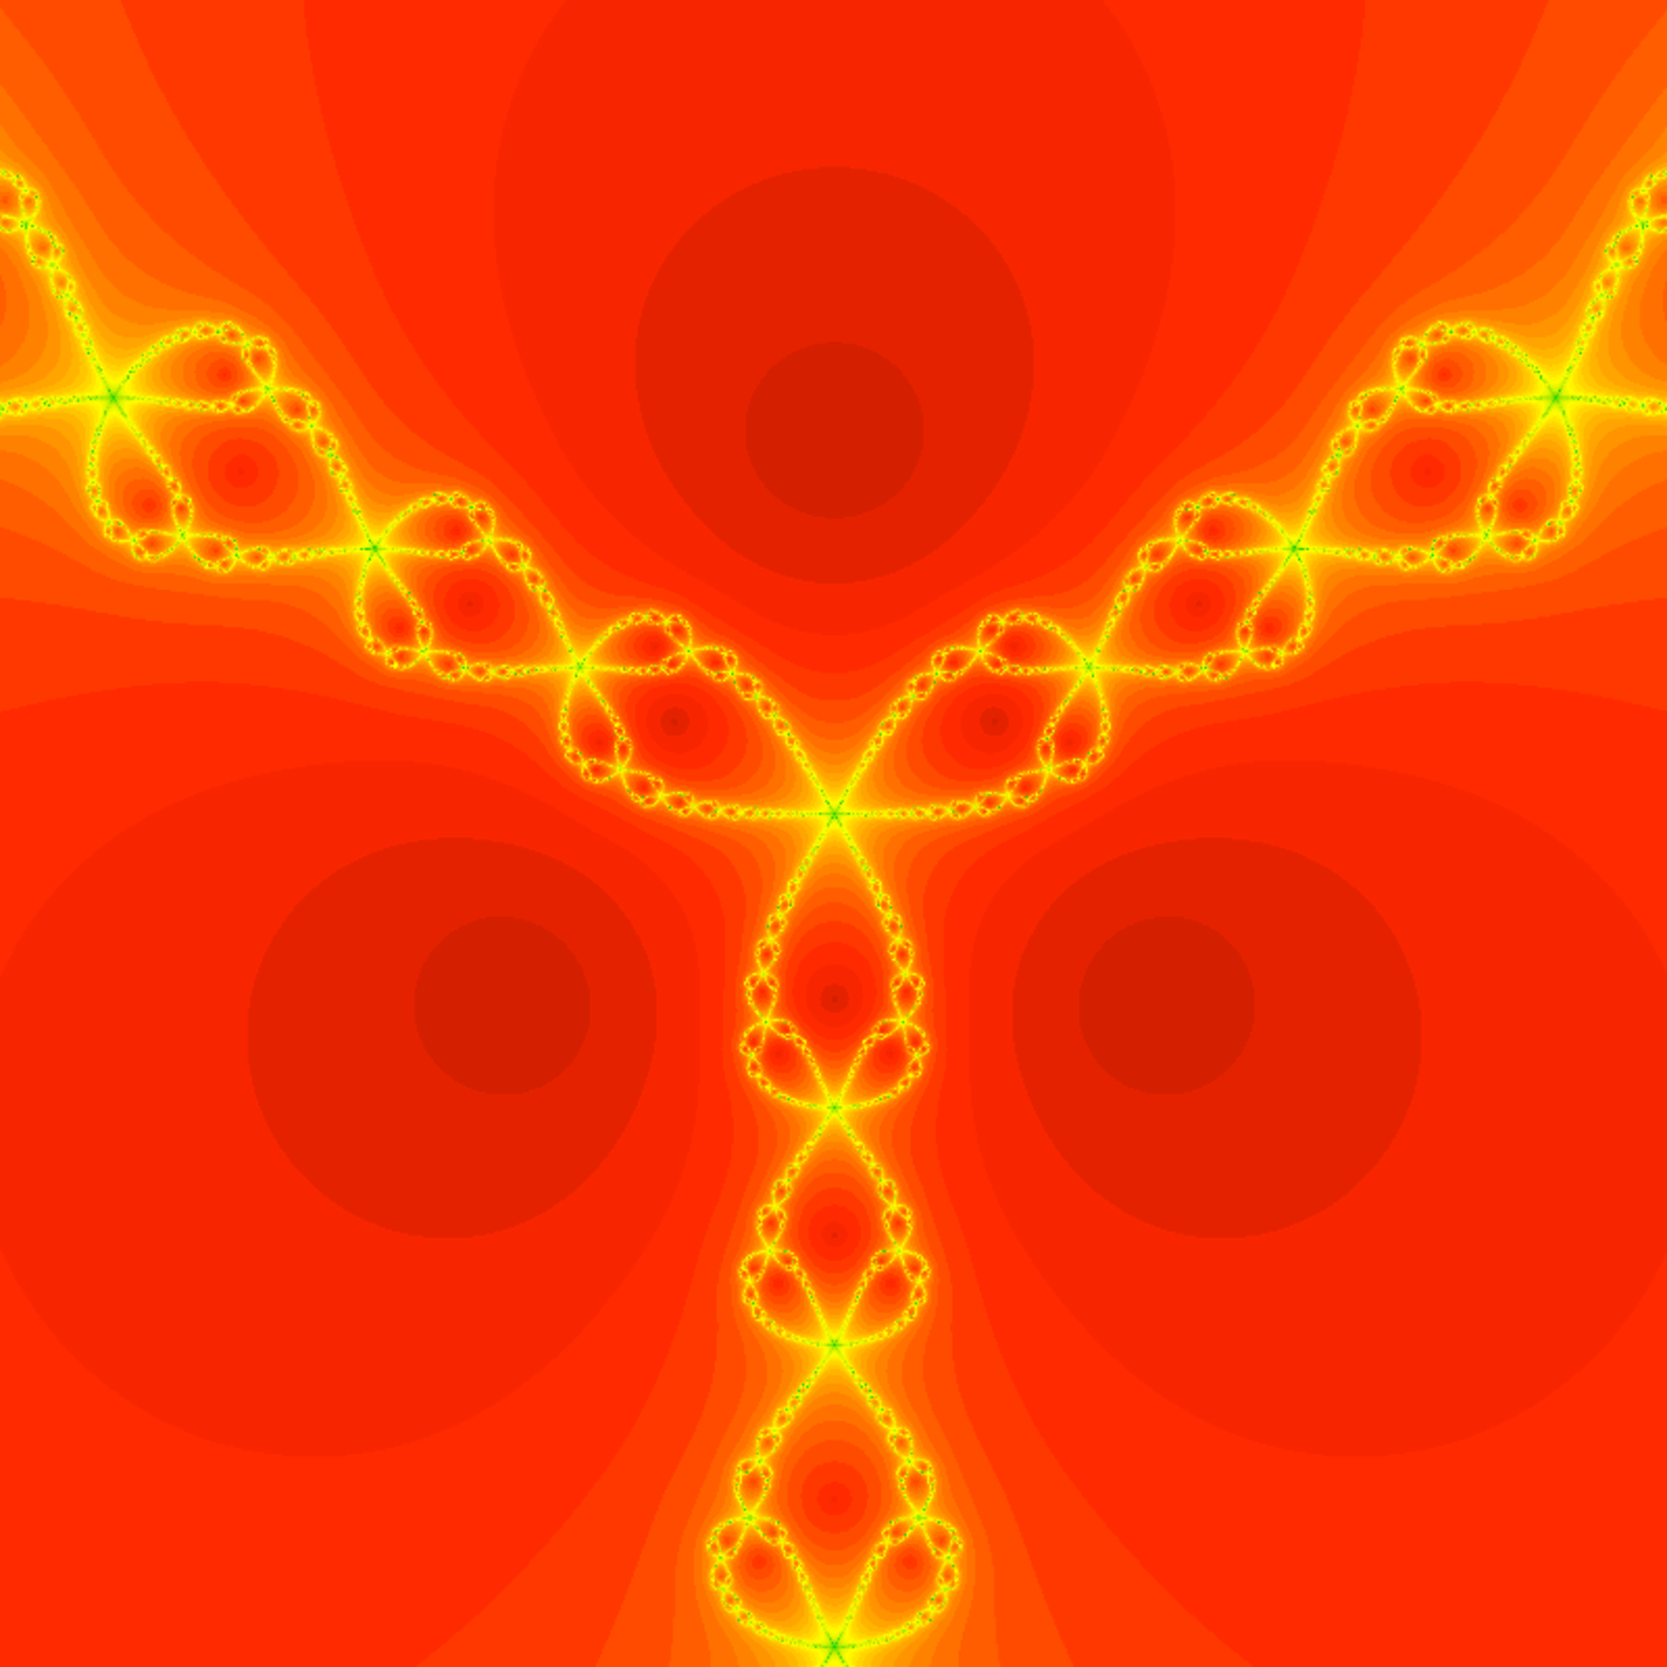
\includegraphics[width=6cm]{samplefigure.pdf}
\end{center}
\caption{\label{sample figure} \small The caption of this figure is ``Newton's method of a cubic polynomial".}
\end{figure}

%%%%%%%%
\section{Mathematics and packages} \label{packages}

By default, the following packages are uploaded:
\begin{enumerate}[\bf (1)]
\item {\tt enumerate:} It allows you to make list with specific somehow arbitrary labels, like this one.
\item {\tt amsthm:} To make evironments with different styles.
\item {\tt amsmath,amssymb,amsfonts:} Multiple mathematics symbols and fonts.
\item {\tt graphicx:} To include figures in a simple and intuitive way.
\item {\tt amscd:} To make commutative diagram with horizontal and vertical arrows. See below.
\item {\tt xy:} To make really fancy commutative arrows. See below.
\item {\tt booktabs:} To make fancy tables.
\end{enumerate}
You may add other standard packages if you need them but try to avoid it if at all possible.

If you need to use them, you will find information about these packages in the usual internet places. 

Here are examples of two commutative diagrams, one made with the package amscd and the other one with xy.

\[
\begin{CD}
A @>g>> B\\
@VV\pi V @VV\pi V\\
X @>f>> Y
\end{CD}
\]


\section{Bibliography}

You may include your references by hand using {\tt the bibliography} (see an example below) or, alternatively, you may use a .bib file and use BibTeX. In any case, we ask you to use a reasonable {\bf consistent} format for all your references. Our recommendation is using BibTex with the style   "plain" or "amsalpha".

%\newpage

\begin{thebibliography}{99}

\bibitem{ex} S.K.\,Agrawal, J.\,Yan. `A three-wheel vehicle with
    expanding wheels: differential flatness, trajectory planning, and control',
    \textit{Proc. of the 2003 IEEWRSJ, Intl. Conference on Intelligent Robots and
    Systems}, Las Vegas, 2003.

\bibitem{ah0} L.~Ahlfors. {\em Complex analysis. An introduction to the theory of analytic functions of one complex variable}, 3rd ed. McGraw-Hill, 1978.

\bibitem{ahl} L.~Ahlfors. {\em Lectures on quasiconformal mappings}, 2nd ed.
University Lecture series {\bf 38}, American Mathematical Society, 2006.

\bibitem{ahlber} L.~Ahlfors and L.~Bers.
  Riemann mapping's theorem for variable metrics,
{\em Annals of Math.}~{\bf 72} (1960), 385--404.
    
\bibitem{CLM89} B.\,Charlet, J.\,L\'evine, R.\,Marino. On dynamic feedback
    linearization, {\em System and Control Letters} \textbf{13} (1989), 143--151.

\end{thebibliography}

%______________________________________________________________
\appendix
\vfill\newpage \section{Title of the appendix}
You can include here an appendix with details that can not be included in the core of the document. You should reference the sections in this appendix in the core document.
\vfill\newpage \section{Title of the appendix}
Second appendix.

\end{document}


